\def\lecturenumber{03}
\documentclass[11pt,a4paper]{article}
\usepackage[T1]{fontenc}
\usepackage[utf8]{inputenc}
\usepackage{lmodern}
\usepackage[margin=19mm,top=21mm,bottom=21mm,headheight=15pt]{geometry}
\usepackage{amsmath,amssymb,booktabs,array,graphicx,microtype}
\usepackage[dvipsnames]{xcolor}
\usepackage{enumitem,fancyhdr,listings,tcolorbox}
\usepackage[colorlinks=true,linkcolor=MidnightBlue,urlcolor=MidnightBlue]{hyperref}
\definecolor{courseblue}{HTML}{164B69}
\definecolor{pale}{HTML}{F0F5F7}
\pagestyle{fancy}
\fancyhf{}
\fancyhead[L]{\small\sffamily\color{courseblue}VALIDATED COMPUTING}
\fancyhead[R]{\small\sffamily Lecture \lecturenumber}
\fancyfoot[L]{\footnotesize Expanded lecture notes \textbullet\ October 2026}
\fancyfoot[R]{\footnotesize\thepage\ / 6}
\renewcommand{\headrulewidth}{0.4pt}
\setlength{\parindent}{0pt}
\setlength{\parskip}{5.5pt plus 1pt}
\setlength{\emergencystretch}{1.5em}
\setlist[itemize]{leftmargin=1.5em,itemsep=3pt,topsep=3pt}
\setlist[enumerate]{leftmargin=1.7em,itemsep=5pt,topsep=4pt}
\lstset{language=Python,basicstyle=\small\ttfamily,keywordstyle=\color{courseblue}\bfseries,
 commentstyle=\color{OliveGreen},stringstyle=\color{BrickRed},showstringspaces=false,
 columns=fullflexible,keepspaces=true,frame=single,rulecolor=\color{black!18},
 backgroundcolor=\color{black!2},aboveskip=6pt,belowskip=6pt,breaklines=true,
 xleftmargin=5pt,xrightmargin=5pt,framesep=5pt}
\newcommand{\R}{\mathbb R}
\newcommand{\fl}{\operatorname{fl}}
\newcommand{\abs}[1]{\left|#1\right|}
\newcommand{\heading}[2]{\section*{\color{courseblue}#1}\vspace{-4pt}{\small\sffamily\color{black!65}#2}\par\vspace{3pt}}
\newcommand{\opening}[2]{{\Large\sffamily\bfseries\color{courseblue}Lecture \lecturenumber\quad #1\par}\vspace{5pt}{\small #2}\par}
\newtcolorbox{question}[1]{colback=pale,colframe=courseblue!55,boxrule=0.4pt,
 arc=1mm,left=7pt,right=7pt,top=4pt,bottom=4pt,title={#1},fonttitle=\bfseries\small,
 coltitle=courseblue,colbacktitle=pale}
\newcommand{\reading}[1]{{\footnotesize\textbf{Reading and notebook.} #1\par}}
\hypersetup{pdfauthor={Validated Computing course},pdfsubject={Expanded introductory lecture notes with questions and exercises}}

\hypersetup{pdftitle={Lecture 03: Conditioning, stability, and cancellation}}
\begin{document}
\opening{Conditioning, stability, and cancellation}{Prerequisites: Lectures 01--02, derivatives, quadratic equations.\newline
Goal: distinguish a sensitive problem from an inaccurate evaluation procedure.}
\heading{1. Which error are we measuring?}{0--14 minutes: a vocabulary check and a worked backward error}
Suppose the mathematical task is $y=f(x)$. The intended input is $x$, the stored
input is $\widetilde x$, and an algorithm returns $\widehat y$. The total error
can be separated exactly as
\[
 \widehat y-f(x)=
 \underbrace{\widehat y-f(\widetilde x)}_{\text{evaluation error at stored input}}
 +\underbrace{f(\widetilde x)-f(x)}_{\text{effect of changing the input}}.
\]
The first term depends on how we compute. The second depends on the mathematical
problem and the input change. A better formula may greatly reduce the first term
without reducing the second.

\textbf{Forward error} measures the difference between computed and desired outputs:
$|\widehat y-f(x)|$, or its ratio to $|f(x)|$ when the denominator is nonzero.
\textbf{Backward error} asks for an input change $\Delta x$ such that
$\widehat y=f(x+\Delta x)$. Its magnitude needs an input scale; if several input
changes work, one may seek the smallest under a specified norm. Not every arbitrary
output belongs to the range of $f$, so such a perturbation need not always exist.

\textbf{Worked example: an approximate square root.} Take exact $a=2$ and the
nonnegative candidate $\widehat y=1.4142$, interpreted as an exact decimal. Set
\[
 \Delta a=\widehat y^2-a=-0.00003836.
\]
Then $\widehat y=\sqrt{a+\Delta a}$ exactly, so this is an absolute backward
error for this answer. Moreover,
\[
 |\widehat y-\sqrt a|
 =\frac{|\widehat y^2-a|}{\widehat y+\sqrt a}.
\]
The denominator explains why a residual can be converted into a forward bound
once enough information about the root is known. With both terms greater than
$1$, the forward error is less than $0.00001918$.

\textbf{Conditioning} describes how exact outputs change under input perturbations.
\textbf{Stability} describes an algorithm's errors; a backward-stable algorithm
produces the exact answer to a nearby admissible problem, with a suitably small
perturbation over its stated input domain. A small backward error for one example
is evidence about that example, not a theorem about every execution.
\begin{question}{Explain the difference}
Can an algorithm be backward stable and still have a large forward error?
Can a well-conditioned problem be solved by a poor algorithm? Give a reason for
each answer, then look for concrete examples on the next three pages.
\end{question}

For a concrete example, let the exact input be $x=1+10^{-20}$ and the task
$f(x)=x-1$. Binary64 stores the input as $1$ and the subtraction returns $0$.
The relative backward error is about $10^{-20}$, but the relative forward error
is one. The computed subtraction is exact on the stored data. The problem is
that a tiny admissible input change removes the entire desired output.

\newpage
\heading{2. Derive a condition number and state its limits}{14--30 minutes: local sensitivity versus a finite bound}
Let $f$ be differentiable at $x$, with $x\ne0$ and $f(x)\ne0$. For a small relative
input change $\eta$, write $\Delta x=x\eta$. The definition of the derivative gives
\[
 f(x+x\eta)=f(x)+f'(x)x\eta+o(\eta),
 \qquad
 \frac{f(x+x\eta)-f(x)}{f(x)}=\frac{xf'(x)}{f(x)}\eta+o(\eta).
\]
This motivates the local relative condition number
\[
 \boxed{\kappa_f(x)=\abs{\frac{xf'(x)}{f(x)}}.}
\]
Roughly, a small relative input error may be amplified by a factor $\kappa_f(x)$.
The formula is asymptotic, not a certified finite-perturbation inequality.
\begin{center}\small
\begin{tabular}{@{}lll@{}}\toprule
Function & Relative condition number & Interpretation\\\midrule
$\sqrt x$, $x>0$ & $1/2$ & Relative changes are locally attenuated\\
$x-1$, $x\ne0,1$ & $|x/(x-1)|$ & Sensitive relatively near its zero\\
$(x-1)^6$, $x\ne0,1$ & $|6x/(x-1)|$ & Strong relative sensitivity near 1\\\bottomrule
\end{tabular}
\end{center}
\textbf{Exact comparison.} For $p(x)=(x-1)^6$, choose $x=1.001$ and
$h=0.000001$ as exact decimals. The relative input change is $h/x\approx9.99\cdot10^{-7}$.
The relative output change is exactly
\[
 \frac{p(x+h)-p(x)}{p(x)}=(1.001)^6-1\approx0.006015.
\]
The local prediction is $\kappa_p(x)h/x=6006(h/x)=0.006$.
It explains the scale but is not the exact change. Notice that the output changes
by roughly $0.6\%$ even if both evaluations are done without arithmetic error.

\textbf{A bound that really covers a finite perturbation.} If $f$ is continuously
differentiable on an interval containing $x$ and $x+h$, and $|f'(t)|\le M$
throughout it, the mean value theorem proves
\[
 |f(x+h)-f(x)|\le M|h|.
\]
If also $|f(x)|\ge m>0$, then the relative change is at most $M|h|/m$.
Both bounds must cover the relevant interval, not just its midpoint.

\begin{question}{Choose an appropriate scale}
At $x=1$, $p(x)=0$, so relative output error and the displayed relative condition
number are undefined. What absolute statement can you make if the uncertain input
satisfies $|x-1|\le10^{-3}$? Does the large nearby relative condition number mean
that the absolute output uncertainty must be large?
\end{question}

\textbf{Absolute conditioning answers a different question.} Locally, the
absolute output change is controlled by $|f'(x)|$ times the absolute input change.
For $f(x)=x-1$, this factor is exactly one, even near $x=1$. There is no conflict
with its large relative condition number: dividing the output error by the tiny
value $|x-1|$ changes the scale of comparison. Always identify the perturbation
model and the error metric before declaring a problem ill-conditioned.

\newpage
\heading{3. Cancellation in an innocent polynomial}{30--47 minutes: Tucker's example, exact reference, and interpretation}
The polynomial in Tucker's Example 1.6.2 has two equivalent forms:
\[
 p(t)=t^6-6t^5+15t^4-20t^3+15t^2-6t+1=(t-1)^6.
\]
Near $t=1$, the expanded terms are of order one while their exact sum is tiny.
At the exact decimal $t=1.001$, the answer is $10^{-18}$. Errors in much larger
intermediate terms can dominate this result. Horner evaluation uses fewer operations,
but its intermediate cancellations do not disappear simply because the operation
count is smaller.

If operands already contain errors, subtraction exposes them:
\[
 (a+e_a)-(b+e_b)-(a-b)=e_a-e_b,\qquad
 \frac{|e_a-e_b|}{|a-b|}\le\frac{|e_a|+|e_b|}{|a-b|}.
\]
The subtraction of the stored operands can even be exact. For instance, two
slightly different real numbers may first round to the same float and then subtract
to exactly zero. The information was lost before the subtraction.
\begin{center}
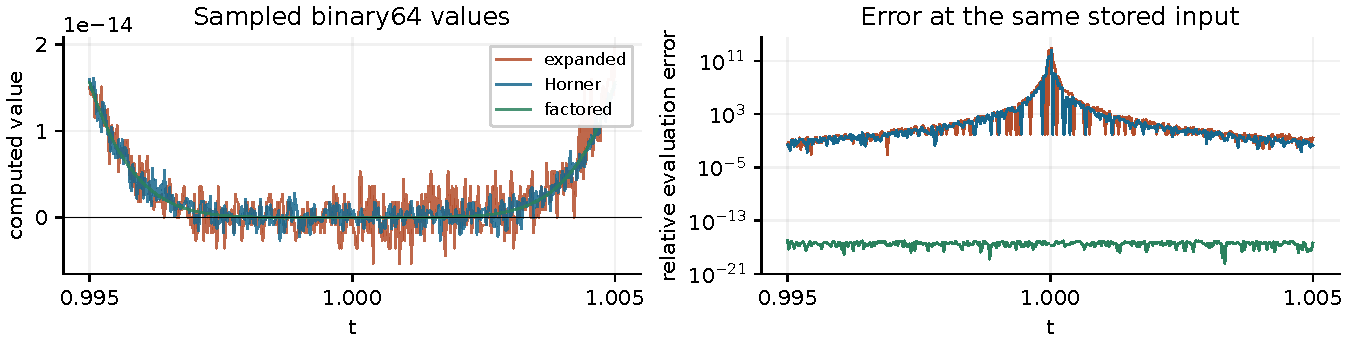
\includegraphics[width=\linewidth]{figures/polynomial_cancellation.pdf}
\end{center}
These are sampled floating-point evaluations, not sign or root certificates.
The algebraic identity proves $p(t)\ge0$ for every real $t$, regardless of any
negative values in the computed graph. The logarithmic error plot omits $t=1$
(relative error is undefined) and samples with exactly zero evaluation error.

To compare algorithms fairly, evaluate the reference at the \emph{same stored input}:
\begin{lstlisting}
from fractions import Fraction
t = 1.001
stored_input = Fraction.from_float(t)
reference = (stored_input - 1)**6
computed = (t - 1)**6
error = abs(Fraction.from_float(computed) - reference)
print(float(error / reference))
\end{lstlisting}
This measures evaluation error without mixing in the conversion of the intended
decimal $1.001$. Factoring can improve that evaluation dramatically; it does not
change the condition number or eliminate uncertainty in the input.
\begin{question}{Explain the apparent contradiction}
How can the factored formula be accurate at the stored float when the problem
is relatively ill-conditioned near $1$? Which term in the page-1 decomposition
has improved, and which has not?
\end{question}

\newpage
\heading{4. Change the formula, preserve the problem}{47--64 minutes: two algebraic repairs and their limitations}
\textbf{Difference of square roots.} For $x\ge0$, rationalization gives
\[
 d(x)=\sqrt{x+1}-\sqrt x
     =\frac{1}{\sqrt{x+1}+\sqrt x}.
\]
The first formula subtracts two close rounded quantities. The second adds them
and takes a reciprocal. At binary64 $x=10^{16}$, even $x+1$ rounds back to $x$,
so the naive result is zero. The reformulated expression gives about $5\cdot10^{-9}$,
which has the correct scale. It is still a rounded approximation, not an enclosure.
For $x>0$, differentiation of the reciprocal form gives
\[
 \kappa_d(x)=\frac12\sqrt{\frac{x}{x+1}}<\frac12.
\]
Thus the loss in the naive formula is not explained by poor relative conditioning
of this mathematical function. It is an algorithmic problem.

\textbf{A small quadratic root.} Consider $x^2+Bx+1=0$ for $B=10^8$.
The usual small-root formula $(-B+\sqrt{B^2-4})/2$ subtracts close numbers.
Compute the large root by addition of same-sign terms, then use the exact identity
$x_1x_2=1$ to obtain the small root:
\begin{lstlisting}
import math
B = 1e8
discriminant = B*B - 4.0
square_root = math.sqrt(discriminant)
naive_small = (-B + square_root) / 2.0
large_root = -0.5 * (B + square_root)
repaired_small = 1.0 / large_root
print(naive_small, repaired_small)
\end{lstlisting}
In the course environment the values are approximately $-7.45\cdot10^{-9}$
and $-10^{-8}$. The naive formula loses about a quarter of the small root's
magnitude. A small absolute error can therefore coexist with a poor relative answer.

For general finite coefficients with $a\ne0$ and discriminant $D>0$, the same idea is
\[
 q=-\tfrac12\bigl(b+\operatorname{copysign}(\sqrt D,b)\bigr),\qquad
 x_1=q/a,\quad x_2=c/q.
\]
Deal separately with linear equations, zero constant term, and repeated roots.
This formula does not by itself prevent overflow in $b^2-4ac$, underflow in a
small root, or an unreliable discriminant sign near a double root.
\begin{question}{Audit before trusting}
Which exact identity justifies the second root? What assumptions make division
by $q$ valid? How would you check the residual of a stored root without trusting
a second floating-point evaluation of the same cancellation-prone expression?
\end{question}

\newpage
\heading{5. Summation order and compensation}{64--78 minutes: inspect a short algorithm and its counterexample}
Floating-point addition is not associative. An explicit left-to-right sum of
$[10^{16},1,-10^{16}]$ gives $0$, whereas the exact sum of these stored inputs is
$1$. Losing a small term early can become decisive after later cancellation.
Use an explicit loop for this experiment: Python's built-in \texttt{sum} need not
implement the naive algorithm below.
\begin{lstlisting}
def naive_sum(values):
    total = 0.0
    for value in values:
        total = total + value
    return total

def kahan_sum(values):
    total = 0.0
    correction = 0.0
    for value in values:
        adjusted = value - correction
        updated = total + adjusted
        correction = (updated - total) - adjusted
        total = updated
    return total
\end{lstlisting}
The compensation variable records low-order information lost in an addition and
feeds it into a later step. Follow one update on paper before thinking of it as a
black box. If adding \texttt{adjusted} leaves \texttt{total} unchanged, the computed
correction becomes approximately its negative, increasing the next adjusted term.

For the list $[1,2^{-54},\ldots,2^{-54}]$ with 10000 small entries, the exact sum
is $1+10000\cdot2^{-54}$. A naive forward loop loses every small term. In this
example, reversing the order, Kahan summation, and \texttt{math.fsum} all recover
the exact representable total. This is a checked example, not a universal exactness claim.

Indeed, the displayed Kahan algorithm still returns zero for
$[10^{16},1,-10^{16}]$. Compensation helps many sums, but does not certify all sums.
For exact stored inputs, a sum of \texttt{Fraction.from\_float} values supplies an
independent rational reference; for general data, rigorous error bounds are needed.

\textbf{Conditioning of the sum itself.} If $s=\sum_i x_i\ne0$ and each input
perturbation satisfies $|\Delta x_i|\le\eta|x_i|$, then
\[
 \frac{|\sum_i(x_i+\Delta x_i)-s|}{|s|}
 \le \eta\,\frac{\sum_i|x_i|}{|s|}.
\]
This inequality is exact. Heavy cancellation in the true sum can make the factor
large even when the summation algorithm is excellent. Stable arithmetic and
well-determined input data solve different parts of the problem.

\newpage
\heading{6. Exercises: diagnose, repair, and justify}{78--90 minutes: discuss one diagnosis and one repair; remaining work is practice}
\begin{enumerate}
\item \textbf{Conditioning with a finite bound.} For $f(x)=x-1$ at
$x=1.000001$, compute the relative condition number. Let $|h|\le10^{-9}$.
Give an exact absolute bound on $|f(x+h)-f(x)|$ and a relative bound using
$|f(x)|$. Explain why an accurate subtraction cannot remove this sensitivity.
\item \textbf{Separate two errors.} For \texttt{t = 1.001}, construct both the
exact decimal input and the exact rational value of the stored float. Compute
$p$ exactly at both. Then compare the expanded, Horner, and factored floating-point
evaluations against the stored-input reference. Use a plain coefficient loop for
Horner's method. Which error does each comparison measure? Why is a negative
computed value not a counterexample to $p(t)\ge0$?
\item \textbf{A useful reformulation.} Rewrite
$\sqrt{1+x}-1$ without subtracting close values, for $x>-1$.
Compare both formulas at $x=10^{-16}$. Derive the relative condition number for
$x\ne0$ and its limit as $x\to0$. Is the inaccurate naive result caused by an
ill-conditioned mathematical problem? Label any high-precision reference as an
approximation unless you also justify a bound.
\item \textbf{Compensation is not certification.} Trace the Kahan code on
$[10^{16},1,-10^{16}]$, writing the values of \texttt{adjusted}, \texttt{updated},
and \texttt{correction}. Identify where information is lost again. Compare with
\texttt{math.fsum} and an exact rational sum. What would you need to certify a
result when exact rational summation is too expensive?
\end{enumerate}
\textbf{Optional extension: a smaller step can be worse.} For $f(x)=x^2$,
the exact forward difference at $1$ is
\[
 D_h=\frac{(1+h)^2-1}{h}=2+h\qquad(h\ne0).
\]
Its truncation error is $|h|$. In machine arithmetic, small numerator errors are
divided by $h$, and sufficiently small $h$ makes $1+h$ round to $1$.
Explain the competing terms in the heuristic model $C_1h+C_2u/h$ for $h>0$.
Its minimum occurs at $h=\sqrt{C_2u/C_1}$ when both constants are positive;
without justified constants, this is guidance rather than a certificate.

\textbf{Selected checks.} Exercise 1 gives $\kappa=1000001$, absolute bound
$10^{-9}$ and relative bound $10^{-3}$. In Exercise 3 the reformulation is
$x/(\sqrt{1+x}+1)$ and
$\kappa=(\sqrt{1+x}+1)/(2\sqrt{1+x})\to1$.
For the page-2 question, $0\le p(x)\le10^{-18}$.

\reading{Companion: \texttt{notebooks/03\_stability.ipynb}; Lab 03: equivalent formulas.
Tucker (2011), \S1.6, especially Example 1.6.2, pp. 20--21. Rump's expression
(Example 1.6.1) is an optional notebook extension. For the summation interface,
see \href{https://docs.python.org/3/library/math.html\#math.fsum}{Python's math.fsum documentation}.}
\end{document}
